\section{Implementation}\label{sec:imp}
Implementation is the last part before testing. It is divided into two parts: frontend Implementation and Database or Backend Implementation. Our coding environment was "VS CODE". It is a trendy code editor authored by Microsoft. For the version controlling system, we used GitHub. GitHub is the best version controlling system in the current world. Our online GitHub repository is located at ''https://github.com/Brainless-Loco/dmbs-project''. We used "Node Package Manager" (npm).
\begin{figure}[H]
	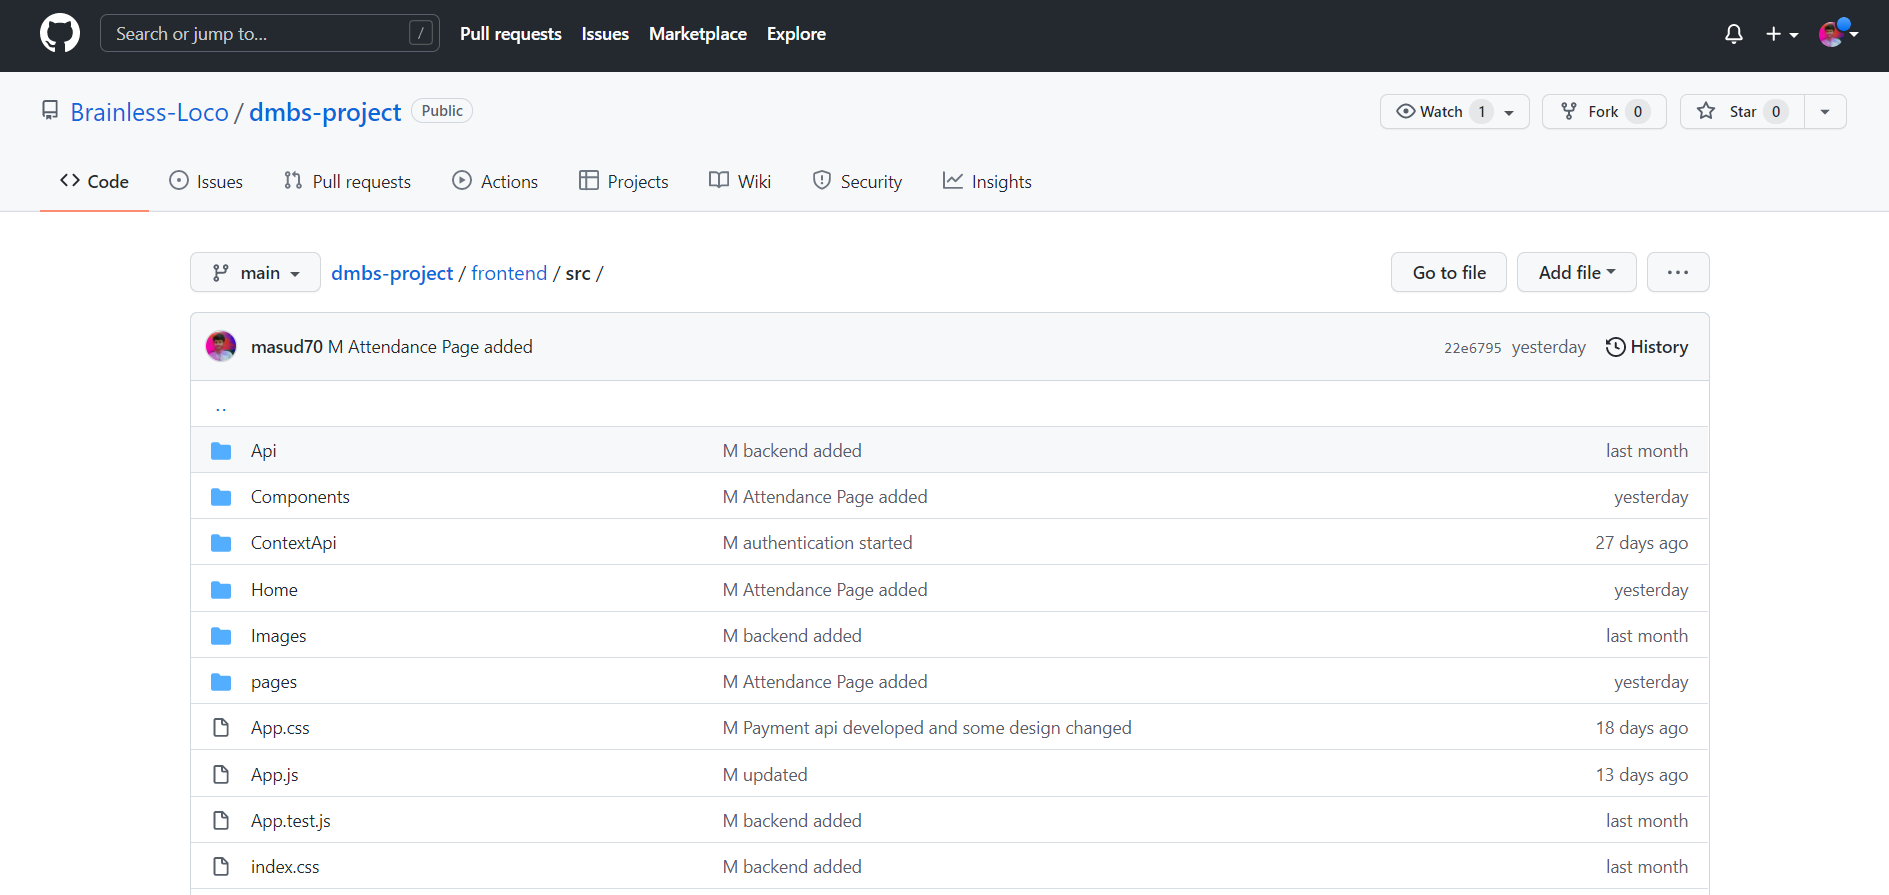
\includegraphics[width=1\textwidth]{images/github}
	\caption{Github repository of CU-OPAS}
\end{figure}

\subsection{Frontend}\label{sub:frontend}
As mentioned before, to implement the frontend, we used Javascript based framework named "React", including various libraries like 'moment js', 'antd', 'material UI', 'react spinners', 'jquery' etc. some of the frontend UI design of our system is mentioned below.

\begin{figure}[H]
	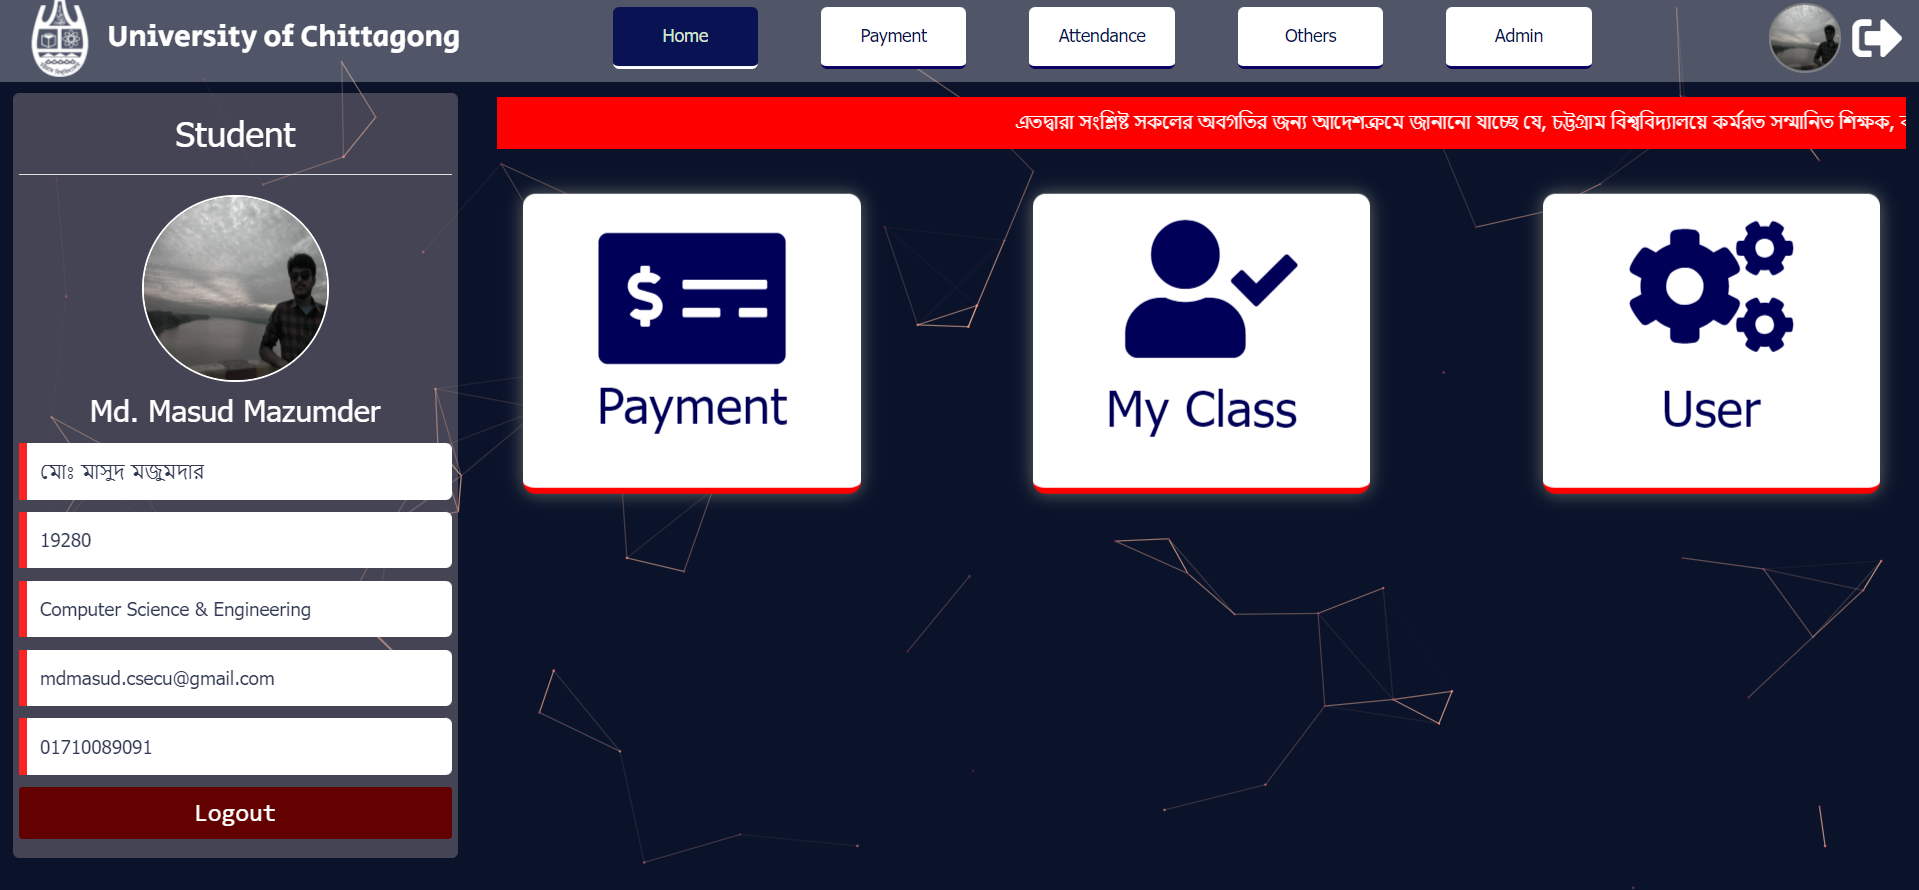
\includegraphics[width=1\textwidth]{images/home}
	\caption{Home Page User Interface}
\end{figure}
\begin{figure}[H]
	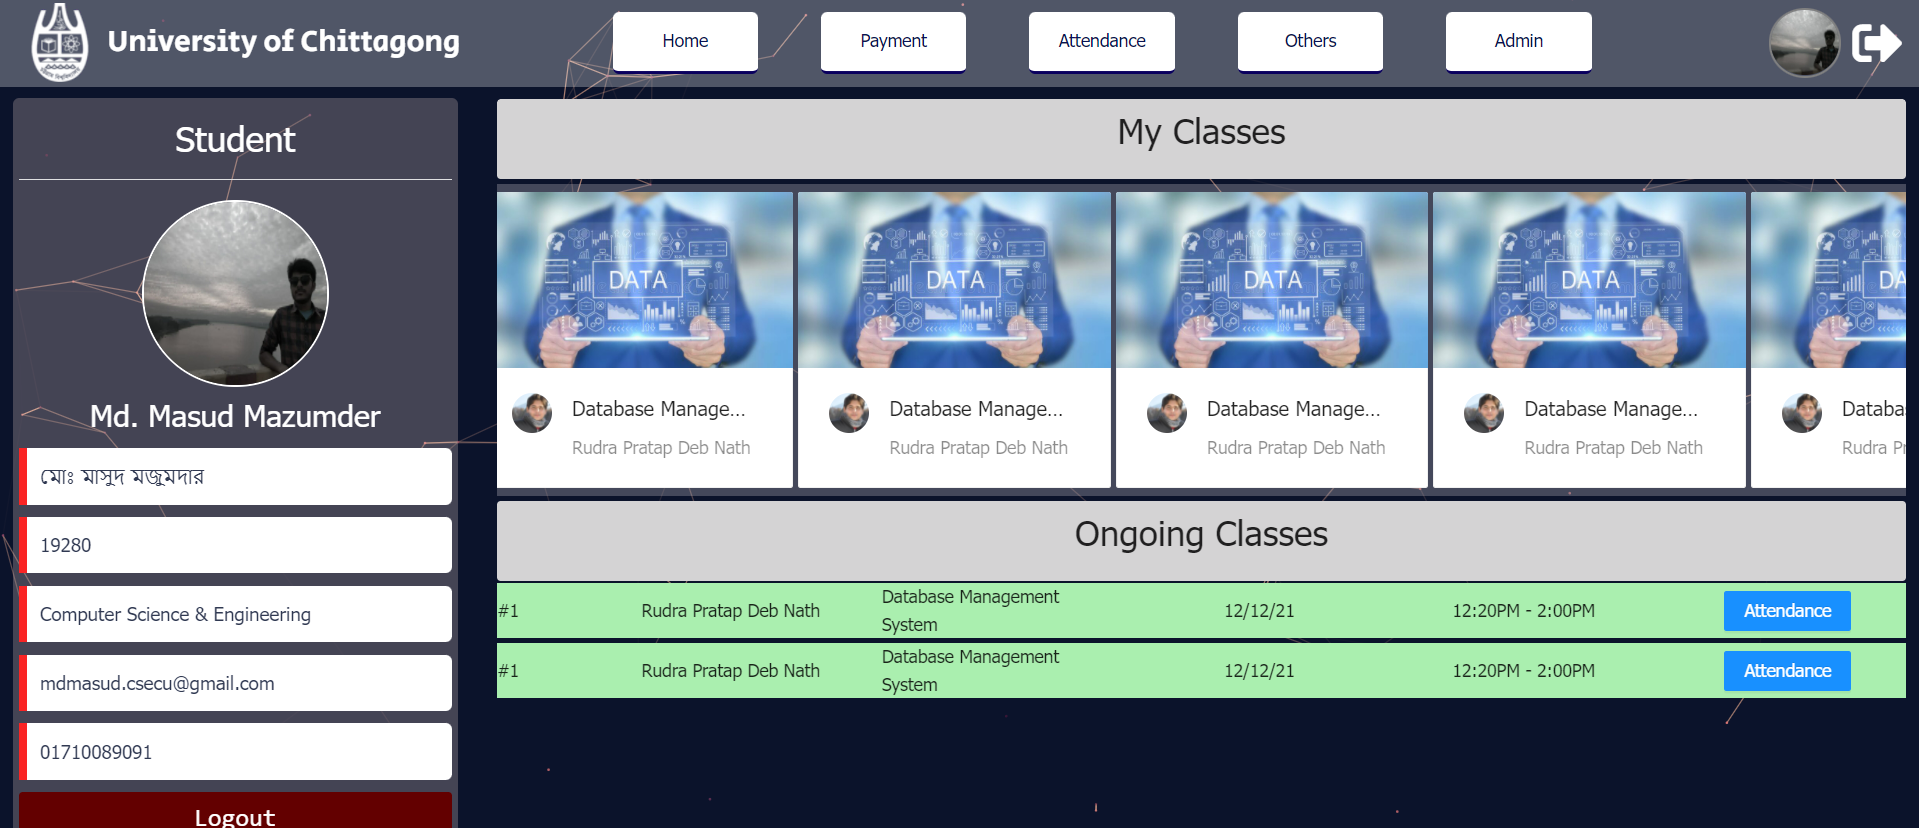
\includegraphics[width=1\textwidth]{images/stu_att}
	\caption{Student Attendance User Interface}
\end{figure}
\begin{figure}[H]
	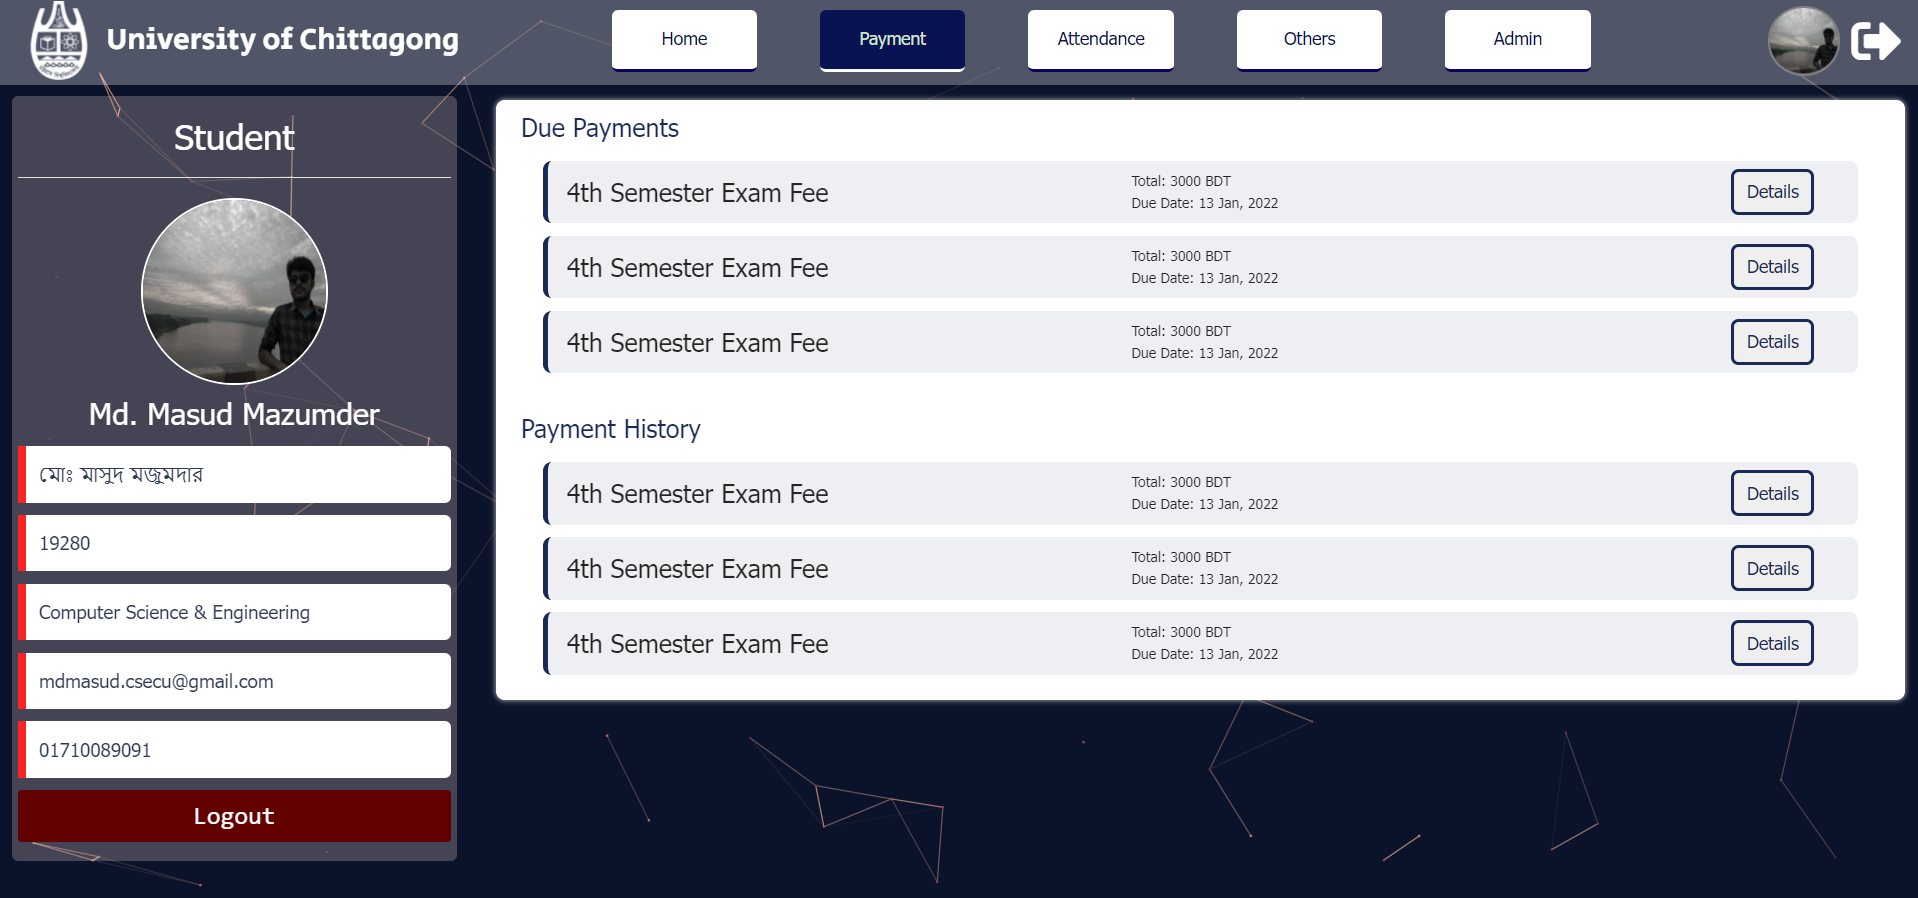
\includegraphics[width=1\textwidth]{images/payhistory}
	\caption{Payment History User Interface}
\end{figure}
\begin{figure}[H]
	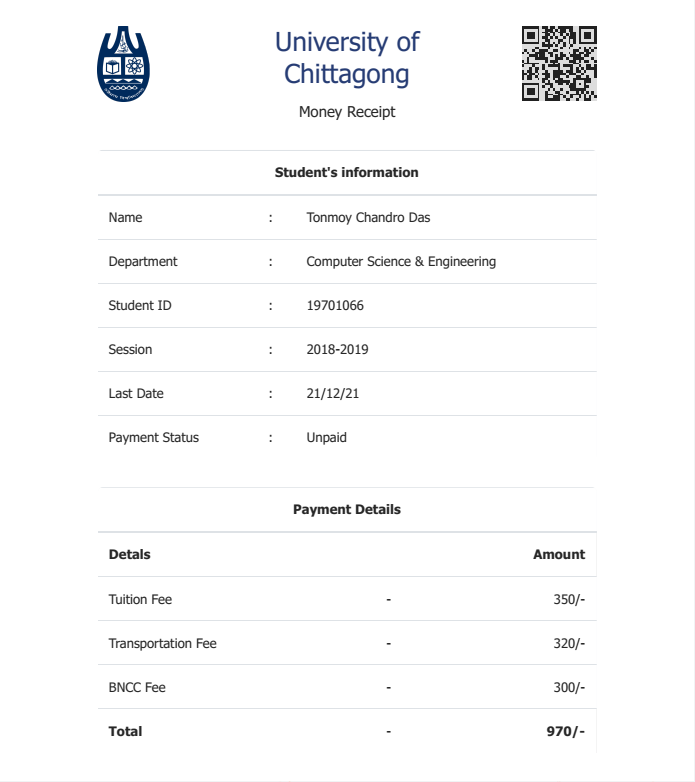
\includegraphics[width=1\textwidth]{images/payslip}
	\caption{Payment Slip}
\end{figure}
\begin{figure}[H]
	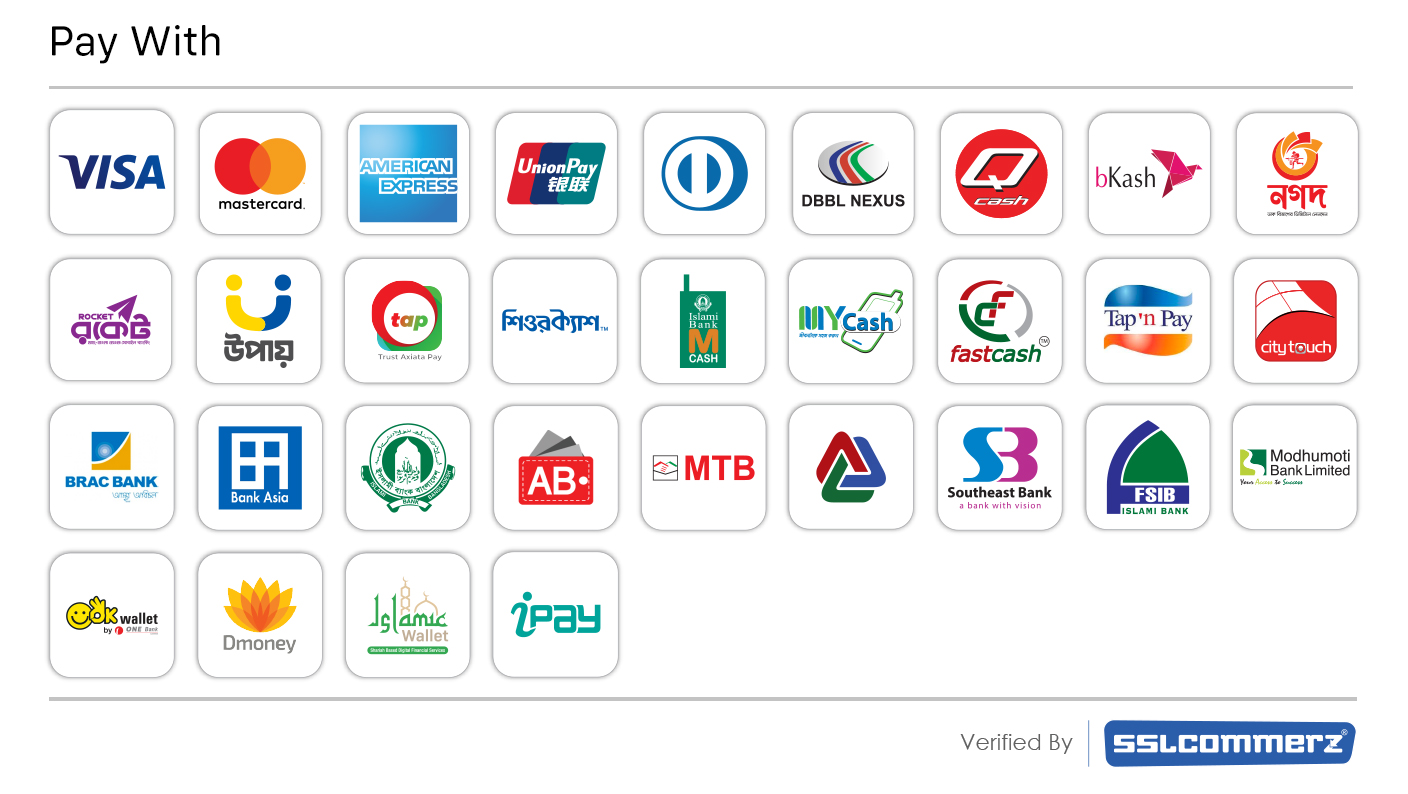
\includegraphics[width=1\textwidth]{images/Payment-Brands}
	\caption{Available Payment Methods}
\end{figure}
\begin{figure}[H]
	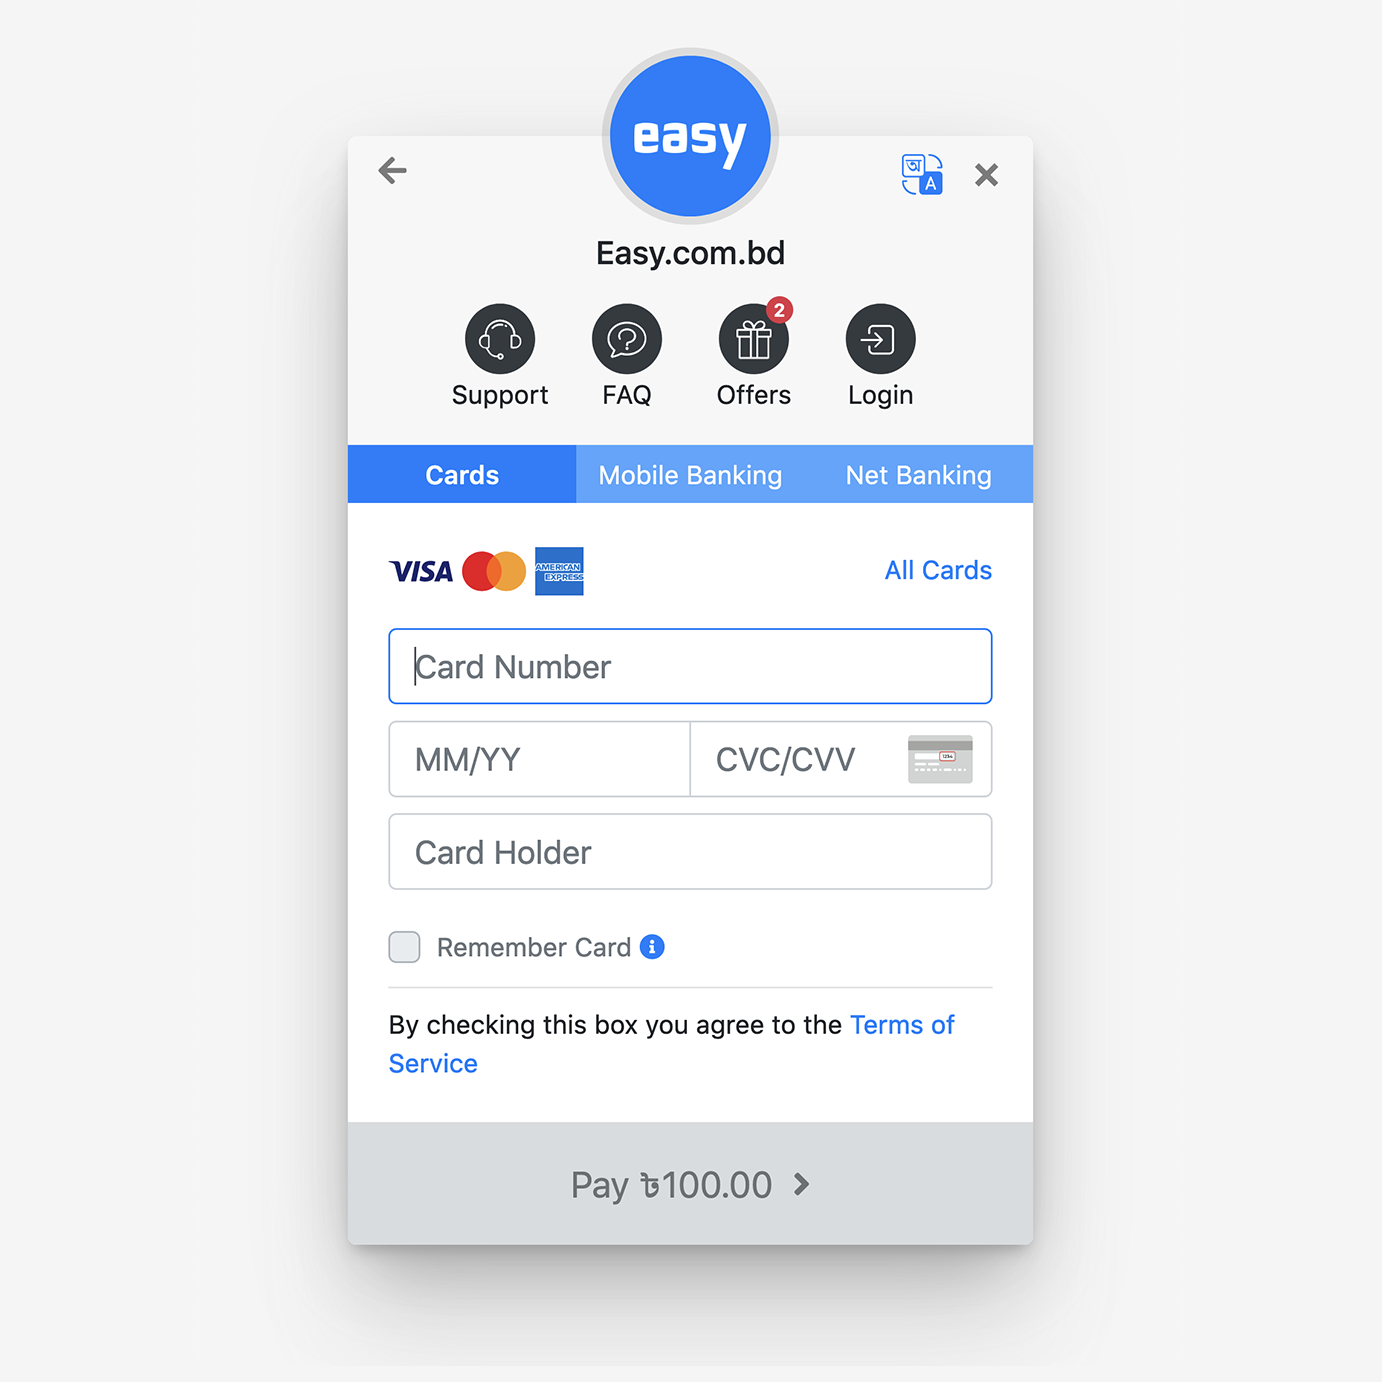
\includegraphics[width=1\textwidth]{images/sslcommerz-card-entry}
	\caption{Payment Procedure}
\end{figure}
\begin{figure}[H]
	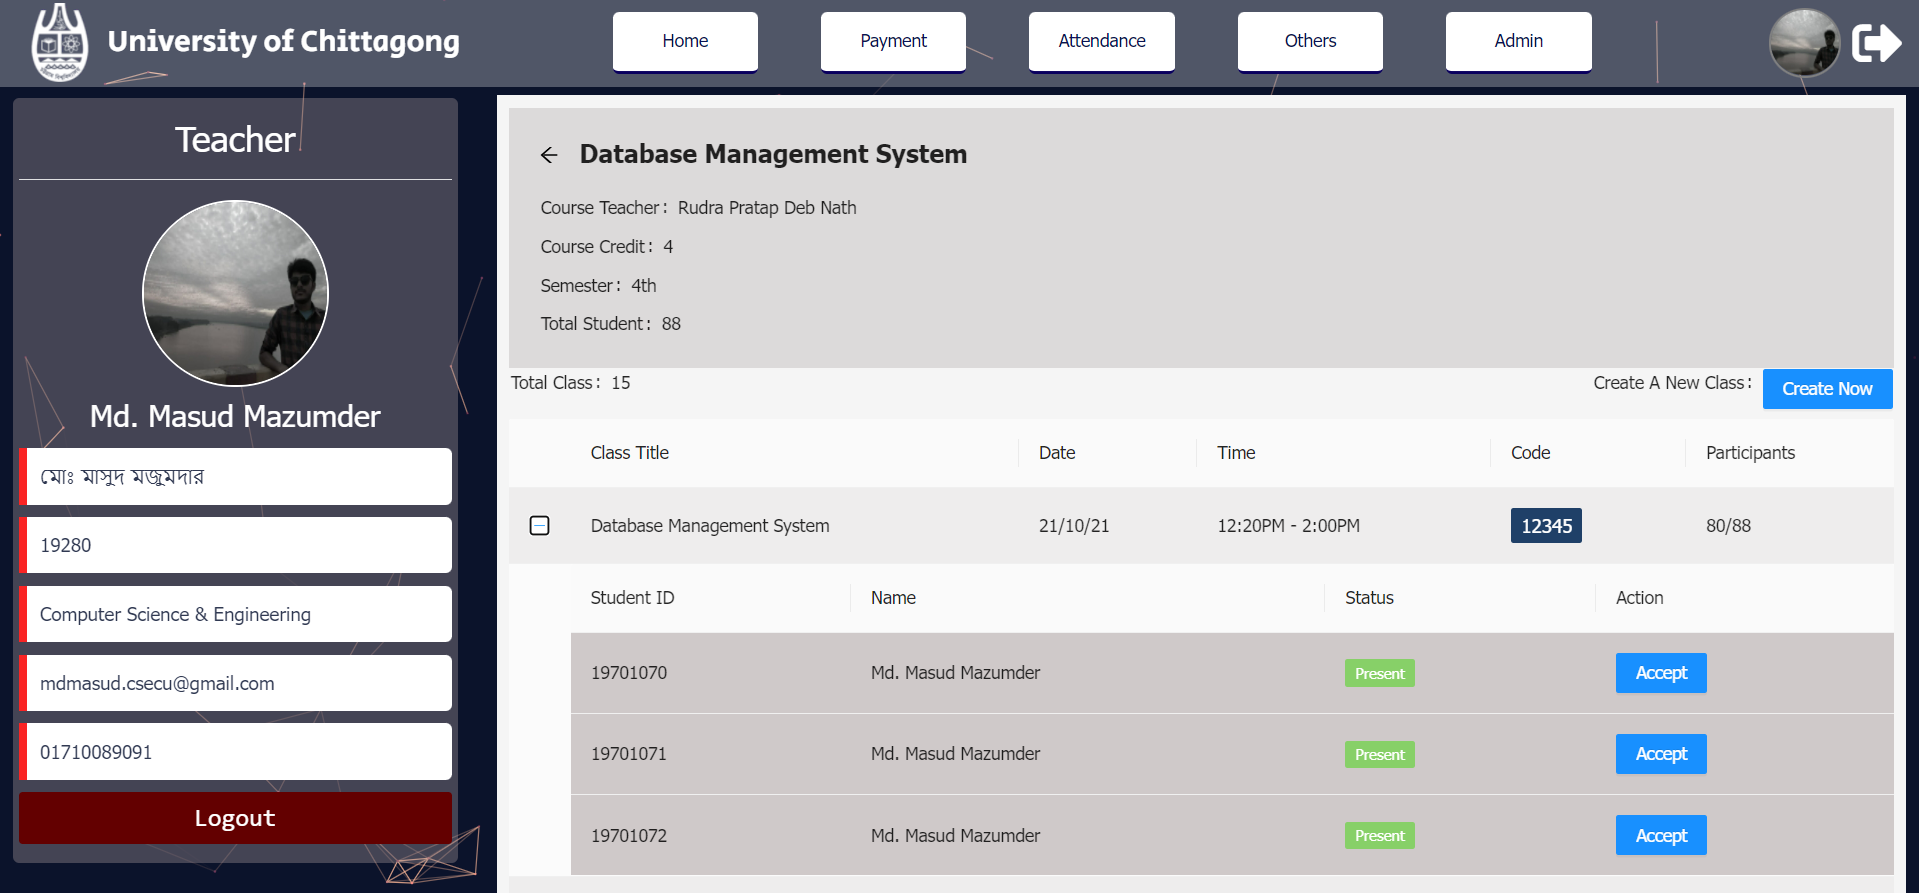
\includegraphics[width=1\textwidth]{images/teacher_att}
	\caption{Teacher Attendance Interface}
\end{figure}
\begin{figure}[H]
	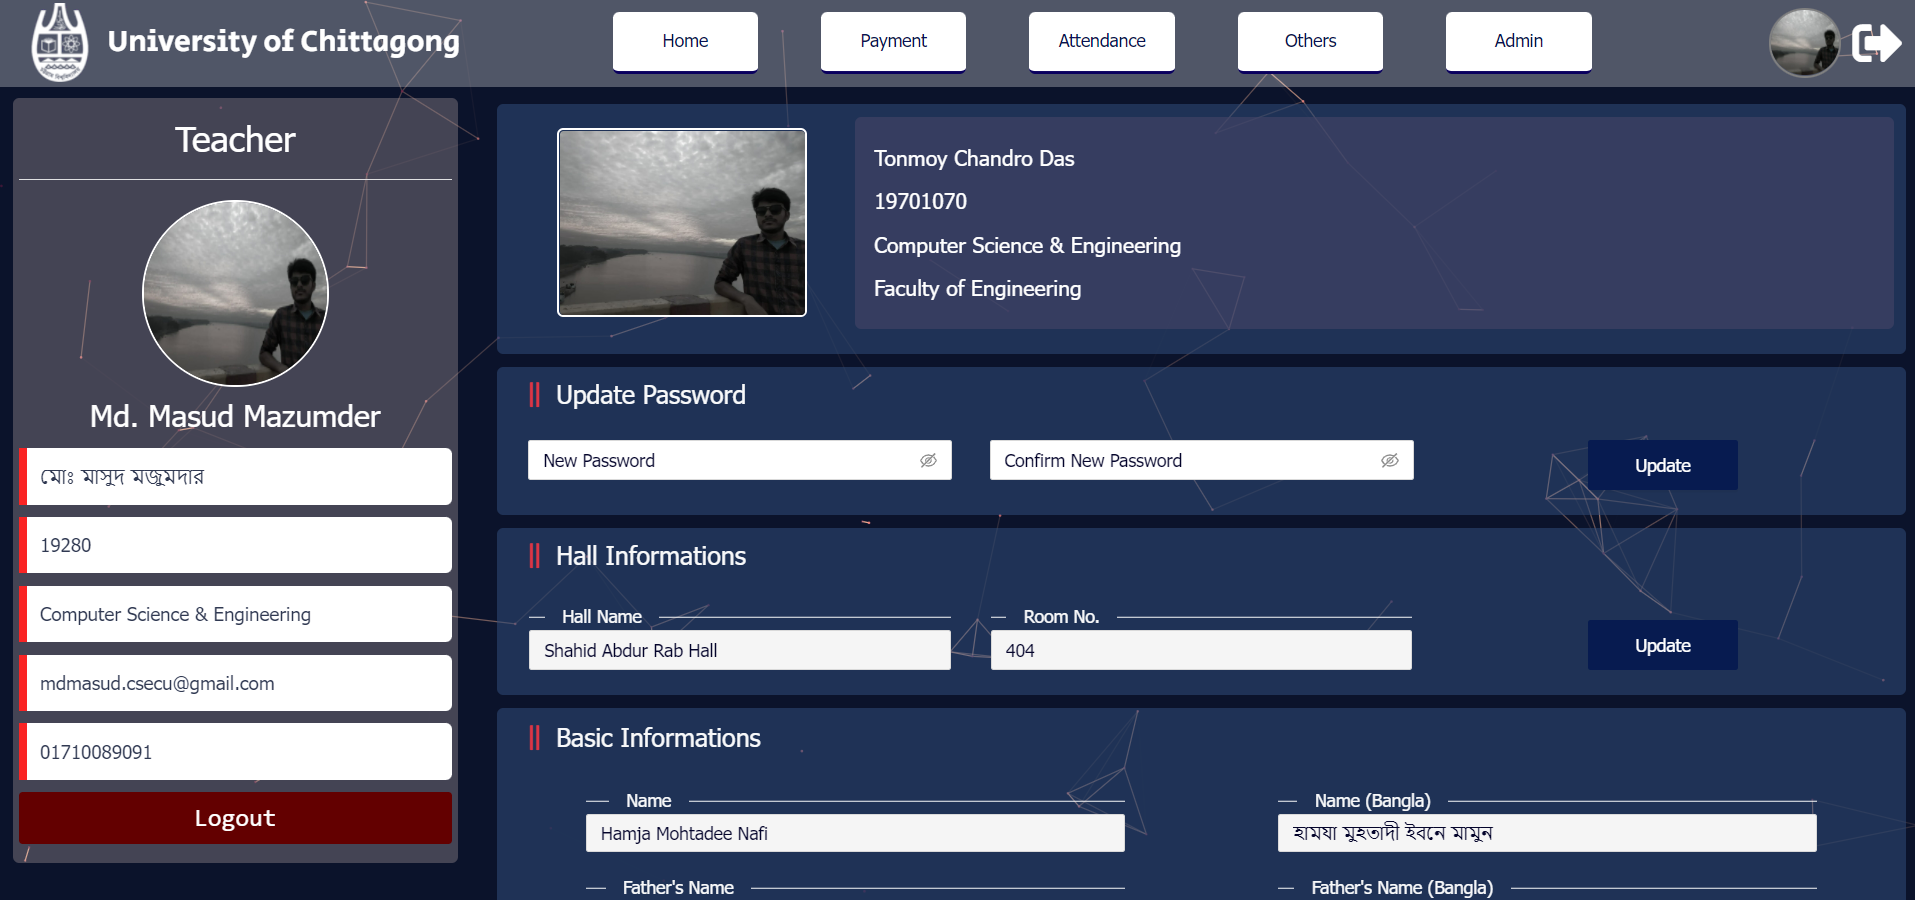
\includegraphics[width=1\textwidth]{images/updateUser}
	\caption{User Update Form}
\end{figure}

\subsection{Database}\label{sub:database}
We implemented our database using the MYSQL server. MYSQL is an open-source relational database that is fast, reliable, and easy to use. It uses a particular query language called "Structured Query Language" or SQL.
Listing~\ref{list:sql} shows an SQL query. 
\begin{lstlisting}[caption={A SQL query to find a User}, label=list:sql, captionpos=b,
           backgroundcolor=\color{white},
           language=SQL,
           breaklines=true,
           frame=single,
           showspaces=false,
           basicstyle=\ttfamily,
           numbers=left,
           numberstyle=\tiny,
           rulecolor=\color{red},
           keywordstyle=\color{blue},
           commentstyle=\color{gray}
        ]
SELECT
    user_id,
    NAME,
    name_bangla,
    email,
    phone,
    dob,
    image,
    religion,
    father,
    mother,
    nationality,
    present_address,
    permanent_address,
    marital_status,
    PASSWORD,
STATUS
    ,
    role,
    department_name
FROM
    USER user_id = 101
\end{lstlisting}
\begin{lstlisting}[caption={A SQL query to find a Student data}, label=list:sql, captionpos=b,
           backgroundcolor=\color{white},
           language=SQL,
           breaklines=true,
           frame=single,
           showspaces=false,
           basicstyle=\ttfamily,
           numbers=left,
           numberstyle=\tiny,
           rulecolor=\color{red},
           keywordstyle=\color{blue},
           commentstyle=\color{gray}
        ]
SELECT
    student_id AS id,
    user_id,
    NAME,
    name_bangla,
    email,
    phone,
    dob,
    image,
    religion,
    father,
    mother,
    nationality,
    present_address,
    permanent_address,
    marital_status,
    PASSWORD,
STATUS
    ,
    role,
    SESSION,
    department_name,
    alloted_hall,
    semester_id
FROM
    student
NATURAL JOIN USER NATURAL JOIN 
department WHERE user_id = 1
\end{lstlisting}
\begin{lstlisting}[caption={A SQL query to insert payment purpose}, label=list:sql, captionpos=b,
           backgroundcolor=\color{white},
           language=SQL,
           breaklines=true,
           frame=single,
           showspaces=false,
           basicstyle=\ttfamily,
           numbers=left,
           numberstyle=\tiny,
           rulecolor=\color{red},
           keywordstyle=\color{blue},
           commentstyle=\color{gray}
        ]
INSERT INTO payment_purpose(
    purpose_title,
    department_id,
    created_by,
    created_at
)
VALUES(?, ?, ?, ?)
\end{lstlisting}
\begin{lstlisting}[caption={A SQL query to find course data}, label=list:sql, captionpos=b,
           backgroundcolor=\color{white},
           language=SQL,
           breaklines=true,
           frame=single,
           showspaces=false,
           basicstyle=\ttfamily,
           numbers=left,
           numberstyle=\tiny,
           rulecolor=\color{red},
           keywordstyle=\color{blue},
           commentstyle=\color{gray}
        ]
SELECT
    *,
    (
    SELECT
        COUNT(*) AS total
    FROM
        student
    NATURAL JOIN semester NATURAL JOIN 
    course WHERE course_id = ?
) AS total
FROM
    semester
NATURAL JOIN course WHERE course_id = ?
\end{lstlisting}
\subsection{Backend}\label{sub:backend}
Also, for backend implementation, we used the Javascript-based framework "Express JS". This is the most popular backend library in the current world. We've also used some dependencies like 'MySql', 'Moment JS', 'bcrypt', 'jsonwebtoken' etc. Some DML code snippets are as below.
\begin{figure}[H]
	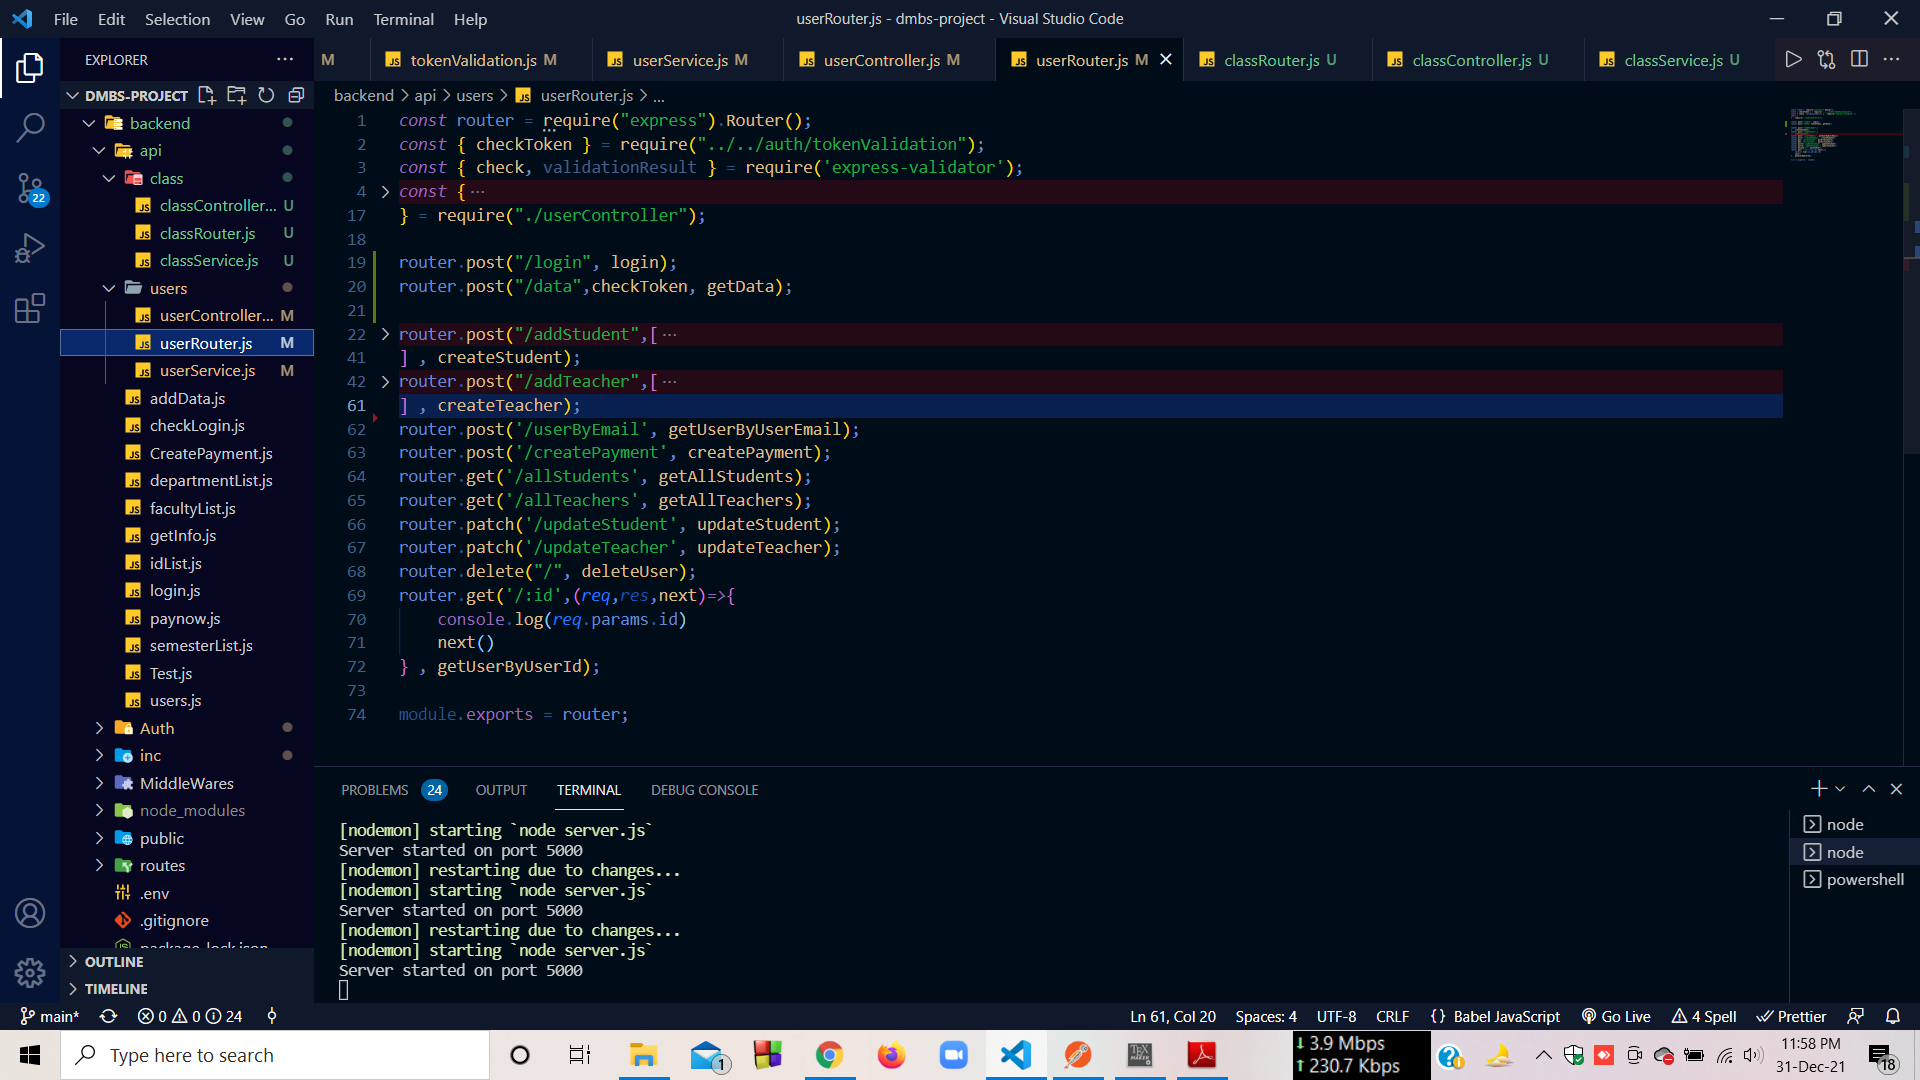
\includegraphics[width=1\textwidth]{images/backend1}
	\caption{Backend API implementation (part-1)}
\end{figure}
\begin{figure}[H]
	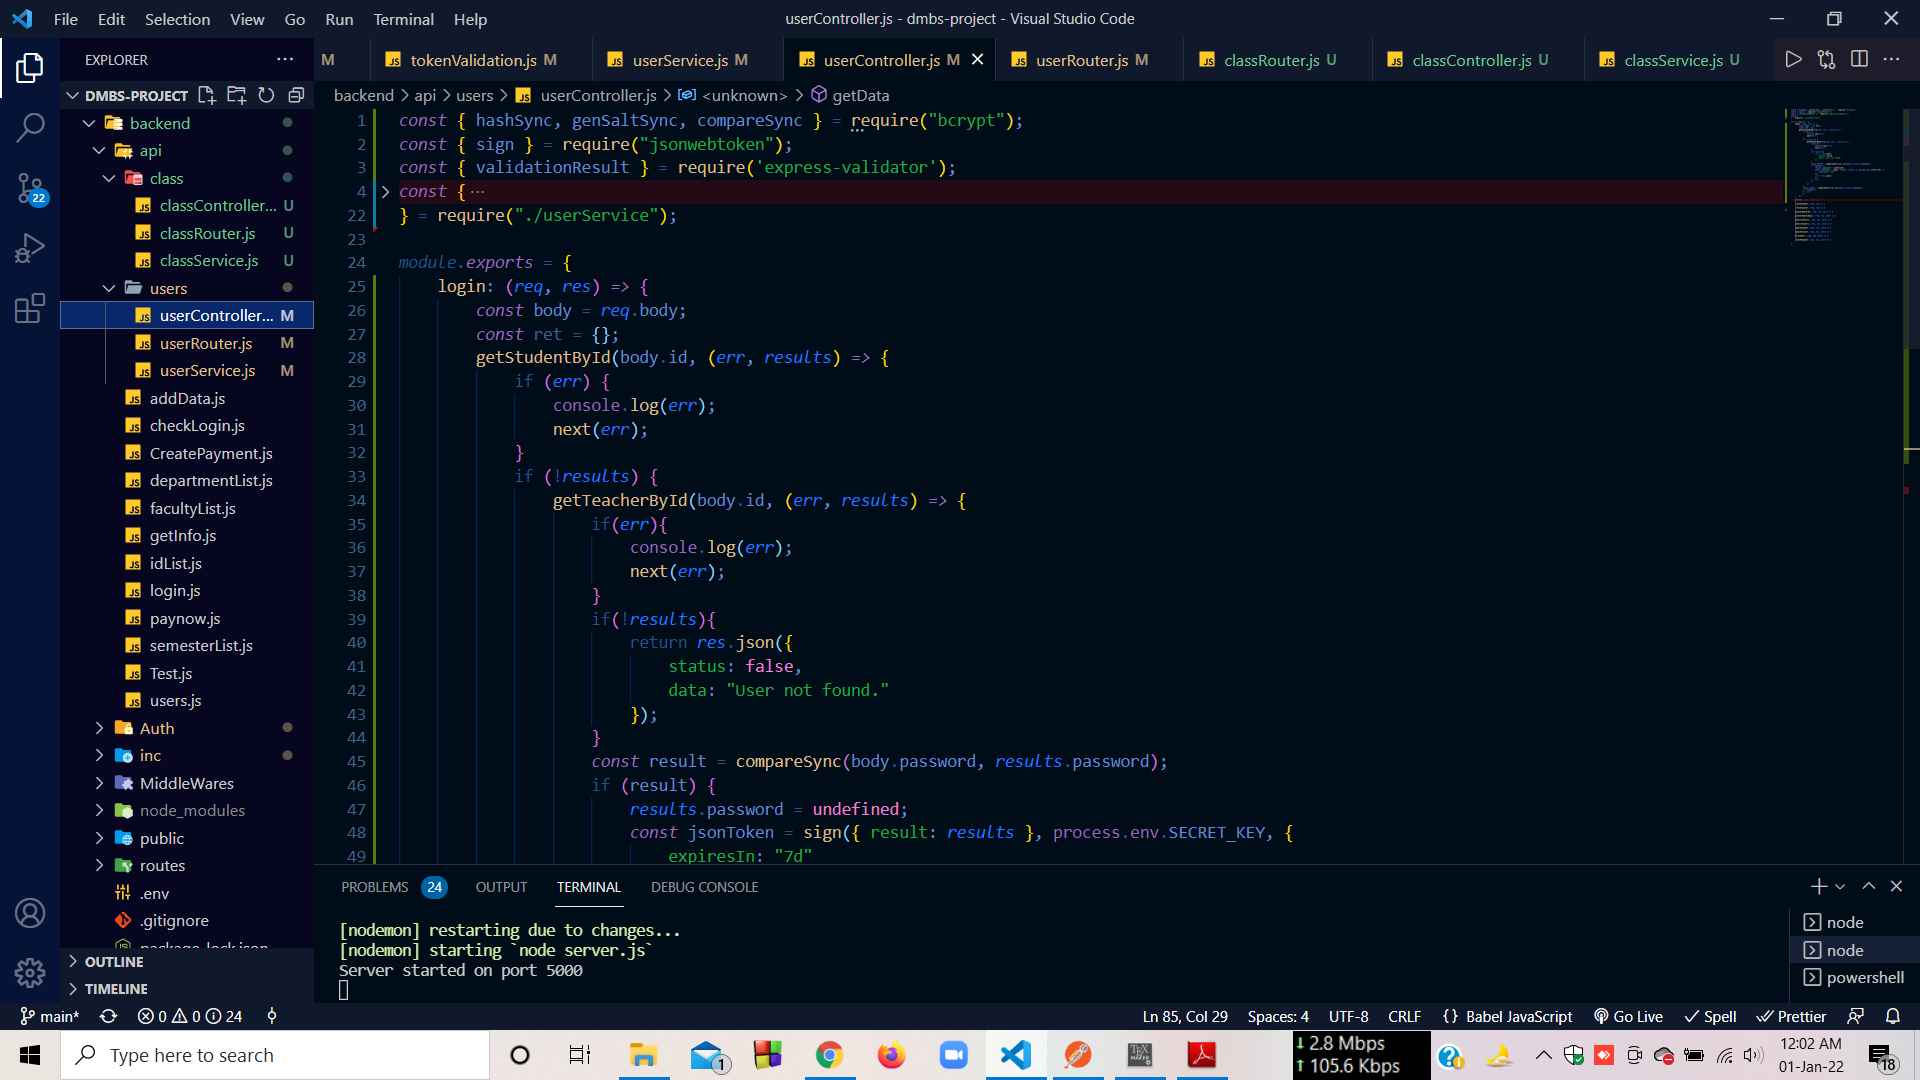
\includegraphics[width=1\textwidth]{images/backend2}
	\caption{Backend API implementation (part-2)}
\end{figure}
\clearpage
